\documentclass[twoside]{book}

% Packages required by doxygen
\usepackage{fixltx2e}
\usepackage{calc}
\usepackage{doxygen}
\usepackage[export]{adjustbox} % also loads graphicx
\usepackage{graphicx}
\usepackage[utf8]{inputenc}
\usepackage{makeidx}
\usepackage{multicol}
\usepackage{multirow}
\PassOptionsToPackage{warn}{textcomp}
\usepackage{textcomp}
\usepackage[nointegrals]{wasysym}
\usepackage[table]{xcolor}

% Font selection
\usepackage[T1]{fontenc}
\usepackage[scaled=.90]{helvet}
\usepackage{courier}
\usepackage{amssymb}
\usepackage{sectsty}
\renewcommand{\familydefault}{\sfdefault}
\allsectionsfont{%
  \fontseries{bc}\selectfont%
  \color{darkgray}%
}
\renewcommand{\DoxyLabelFont}{%
  \fontseries{bc}\selectfont%
  \color{darkgray}%
}
\newcommand{\+}{\discretionary{\mbox{\scriptsize$\hookleftarrow$}}{}{}}

% Page & text layout
\usepackage{geometry}
\geometry{%
  a4paper,%
  top=2.5cm,%
  bottom=2.5cm,%
  left=2.5cm,%
  right=2.5cm%
}
\tolerance=750
\hfuzz=15pt
\hbadness=750
\setlength{\emergencystretch}{15pt}
\setlength{\parindent}{0cm}
\setlength{\parskip}{3ex plus 2ex minus 2ex}
\makeatletter
\renewcommand{\paragraph}{%
  \@startsection{paragraph}{4}{0ex}{-1.0ex}{1.0ex}{%
    \normalfont\normalsize\bfseries\SS@parafont%
  }%
}
\renewcommand{\subparagraph}{%
  \@startsection{subparagraph}{5}{0ex}{-1.0ex}{1.0ex}{%
    \normalfont\normalsize\bfseries\SS@subparafont%
  }%
}
\makeatother

% Headers & footers
\usepackage{fancyhdr}
\pagestyle{fancyplain}
\fancyhead[LE]{\fancyplain{}{\bfseries\thepage}}
\fancyhead[CE]{\fancyplain{}{}}
\fancyhead[RE]{\fancyplain{}{\bfseries\leftmark}}
\fancyhead[LO]{\fancyplain{}{\bfseries\rightmark}}
\fancyhead[CO]{\fancyplain{}{}}
\fancyhead[RO]{\fancyplain{}{\bfseries\thepage}}
\fancyfoot[LE]{\fancyplain{}{}}
\fancyfoot[CE]{\fancyplain{}{}}
\fancyfoot[RE]{\fancyplain{}{\bfseries\scriptsize Generated by Doxygen }}
\fancyfoot[LO]{\fancyplain{}{\bfseries\scriptsize Generated by Doxygen }}
\fancyfoot[CO]{\fancyplain{}{}}
\fancyfoot[RO]{\fancyplain{}{}}
\renewcommand{\footrulewidth}{0.4pt}
\renewcommand{\chaptermark}[1]{%
  \markboth{#1}{}%
}
\renewcommand{\sectionmark}[1]{%
  \markright{\thesection\ #1}%
}

% Indices & bibliography
\usepackage{natbib}
\usepackage[titles]{tocloft}
\setcounter{tocdepth}{3}
\setcounter{secnumdepth}{5}
\makeindex

% Hyperlinks (required, but should be loaded last)
\usepackage{ifpdf}
\ifpdf
  \usepackage[pdftex,pagebackref=true]{hyperref}
\else
  \usepackage[ps2pdf,pagebackref=true]{hyperref}
\fi
\hypersetup{%
  colorlinks=true,%
  linkcolor=blue,%
  citecolor=blue,%
  unicode%
}

% Custom commands
\newcommand{\clearemptydoublepage}{%
  \newpage{\pagestyle{empty}\cleardoublepage}%
}

\usepackage{caption}
\captionsetup{labelsep=space,justification=centering,font={bf},singlelinecheck=off,skip=4pt,position=top}

%===== C O N T E N T S =====

\begin{document}

% Titlepage & ToC
\hypersetup{pageanchor=false,
             bookmarksnumbered=true,
             pdfencoding=unicode
            }
\pagenumbering{roman}
\begin{titlepage}
\vspace*{7cm}
\begin{center}%
{\Large Projekt 3 }\\
\vspace*{1cm}
{\large Generated by Doxygen 1.8.11}\\
\end{center}
\end{titlepage}
\clearemptydoublepage
\tableofcontents
\clearemptydoublepage
\pagenumbering{arabic}
\hypersetup{pageanchor=true}

%--- Begin generated contents ---
\chapter{Projekt 3}
\label{index}\hypertarget{index}{}\hypertarget{index_intro_sec}{}\section{Hash\+Set}\label{index_intro_sec}
\hyperlink{class_hash_set}{Hash\+Set} to kolekcja unikatowych elementow ktora wykorzystuje funkcje \textquotesingle{}hashujaca\textquotesingle{} Rozwiazaniem jest tablica list jednokierunkowych. Numer komorki do ktorej trafi element jest obliczany za pomoca funkcji \textquotesingle{}hashujacej\textquotesingle{}. Jesli napotkany element juz istnieje nie jest on dodawany. Na samym poczatku wszystkie komorki sa puste. Uzycie szablonu pozwala na uzywanie elementow roznego typu(int, string, float itp.). \hypertarget{index_intro_sec3}{}\section{Metody i operatory}\label{index_intro_sec3}
Opisane jest to w zakladce \hyperlink{class_hash_set}{Hash\+Set} $\ast$\hypertarget{index_intro_sec4}{}\section{Mieszkanie}\label{index_intro_sec4}
\hypertarget{index_step1}{}\subsection{Przeglad}\label{index_step1}
\hyperlink{class_mieszkanie}{Mieszkanie} jest klasa reprezentujaca mieszkanie. Pola jakie zawiera klasa \+: \begin{DoxyItemize}
\item string {\bfseries nazw\+Wlasciciela} -\/ nazwa wlasciciela mieszkania\item float {\bfseries powierzchnia} -\/ powierzchnia mieszkania\item int {\bfseries liczba\+Pokoi} -\/ liczba pokoi w mieszkaniu\item bool {\bfseries zamieszkane} -\/ mowi o tym czy mieszkanie jest zamieszkane czy puste \item static unsigned {\bfseries liczba\+Wczytanych\+Mieszk} -\/ licznik poprawnie wczytanych obiektów mieszkań ze strumieni \end{DoxyItemize}
\hypertarget{index_intro_sec10}{}\section{Metody i operatory}\label{index_intro_sec10}
Opisane jest to w zakladce \hyperlink{class_mieszkanie}{Mieszkanie}.\hypertarget{index_intro_sec5}{}\section{Bucket}\label{index_intro_sec5}
\hypertarget{index_step1}{}\subsection{Przeglad}\label{index_step1}
\hyperlink{struct_bucket}{Bucket} jest struktura ktora umozliwia tworzenie listy jednokierunkowej do ktorej dodawana sa elementy w odpowiednich komorkach tablicy. \hypertarget{index_intro_sec10}{}\section{Metody i operatory}\label{index_intro_sec10}
Opisane jest to w zakladce \hyperlink{struct_bucket}{Bucket}. \hypertarget{index_intro_sec9}{}\section{Co zostalo dodane}\label{index_intro_sec9}
Do projektu 2 dodałem dwie klasy pochodne\+: \begin{DoxyItemize}
\item finalna \hyperlink{class_mieszkanie_hipoteczne}{Mieszkanie\+Hipoteczne}\item \hyperlink{class_mieszkanie_wynajmowane}{Mieszkanie\+Wynajmowane}\item a także wirtualna klase bazowa \hyperlink{class_siedziba}{Siedziba}\end{DoxyItemize}
W mainie pokazalem przykladowe rzutowanie w dol i w gore, wskazniki na obiekty. Oczywiscie zgodnie z wymogiem uzylem dodatkowo slowa kluczowego protected w klasie \hyperlink{class_siedziba}{Siedziba}.\hypertarget{index_intro_sec6}{}\section{Obsluga sytuacji wyjatkowych\+:}\label{index_intro_sec6}
Została zastosowana przy uzyciu funkcji remove(). Przy probie usuniecia nieistniejacego obiektu, rzucany jest obiekt typu T.\hypertarget{index_intro_sec7}{}\section{Iterator\+:}\label{index_intro_sec7}
Zostala utworzona klasa iteratora, ktora zostala zaimplementowana z pliku z Hash\+Setem. Zawiera funkce zgodne z zalozeniami projektu(next, prev, begin, end...) \hypertarget{index_intro_sec8}{}\section{Operatory strumieniowe w klasach\+:}\label{index_intro_sec8}
W klasie \hyperlink{class_siedziba}{Siedziba} zostal przeciazony operator $<$$<$ W klasie \hyperlink{class_mieszkanie_wynajmowane}{Mieszkanie\+Wynajmowane} zostaly przeciazone operatory $<$$<$,$>$$>$ W klasie \hyperlink{class_mieszkanie_hipoteczne}{Mieszkanie\+Hipoteczne} nie przeciazylem zadnych operatorow w celu pokazania efektu 
\chapter{Hierarchical Index}
\section{Class Hierarchy}
This inheritance list is sorted roughly, but not completely, alphabetically\+:\begin{DoxyCompactList}
\item \contentsline{section}{Bucket$<$ T $>$}{\pageref{struct_bucket}}{}
\item \contentsline{section}{Hash\+Set$<$ T $>$}{\pageref{class_hash_set}}{}
\item \contentsline{section}{List\+Iterator$<$ T $>$}{\pageref{class_list_iterator}}{}
\item \contentsline{section}{Siedziba}{\pageref{class_siedziba}}{}
\begin{DoxyCompactList}
\item \contentsline{section}{Mieszkanie}{\pageref{class_mieszkanie}}{}
\begin{DoxyCompactList}
\item \contentsline{section}{Mieszkanie\+Hipoteczne}{\pageref{class_mieszkanie_hipoteczne}}{}
\item \contentsline{section}{Mieszkanie\+Wynajmowane}{\pageref{class_mieszkanie_wynajmowane}}{}
\end{DoxyCompactList}
\end{DoxyCompactList}
\end{DoxyCompactList}

\chapter{Class Index}
\section{Class List}
Here are the classes, structs, unions and interfaces with brief descriptions\+:\begin{DoxyCompactList}
\item\contentsline{section}{\hyperlink{struct_bucket}{Bucket$<$ T $>$} \\*Struktura \hyperlink{struct_bucket}{Bucket} }{\pageref{struct_bucket}}{}
\item\contentsline{section}{\hyperlink{class_hash_set}{Hash\+Set$<$ T $>$} \\*Klasa \hyperlink{class_hash_set}{Hash\+Set} }{\pageref{class_hash_set}}{}
\item\contentsline{section}{\hyperlink{class_list_iterator}{List\+Iterator$<$ T $>$} \\*Klasa iteratora }{\pageref{class_list_iterator}}{}
\item\contentsline{section}{\hyperlink{class_mieszkanie}{Mieszkanie} \\*Klasa reprezentujaca mieszkanie }{\pageref{class_mieszkanie}}{}
\item\contentsline{section}{\hyperlink{class_mieszkanie_hipoteczne}{Mieszkanie\+Hipoteczne} \\*Klasa \hyperlink{class_mieszkanie_hipoteczne}{Mieszkanie\+Hipoteczne} }{\pageref{class_mieszkanie_hipoteczne}}{}
\item\contentsline{section}{\hyperlink{class_mieszkanie_wynajmowane}{Mieszkanie\+Wynajmowane} \\*Klasa \hyperlink{class_mieszkanie_wynajmowane}{Mieszkanie\+Wynajmowane} }{\pageref{class_mieszkanie_wynajmowane}}{}
\item\contentsline{section}{\hyperlink{class_siedziba}{Siedziba} \\*Klasa abstrakcyjna \hyperlink{class_siedziba}{Siedziba} }{\pageref{class_siedziba}}{}
\end{DoxyCompactList}

\chapter{Class Documentation}
\hypertarget{struct_bucket}{}\section{Bucket$<$ T $>$ Struct Template Reference}
\label{struct_bucket}\index{Bucket$<$ T $>$@{Bucket$<$ T $>$}}


Struktura \hyperlink{struct_bucket}{Bucket}.  




{\ttfamily \#include $<$Hash\+Set.\+h$>$}

\subsection*{Public Attributes}
\begin{DoxyCompactItemize}
\item 
T \hyperlink{struct_bucket_a3d67ed4728216cb914ce1c06857572e5}{s}\hypertarget{struct_bucket_a3d67ed4728216cb914ce1c06857572e5}{}\label{struct_bucket_a3d67ed4728216cb914ce1c06857572e5}

\begin{DoxyCompactList}\small\item\em Element struktury. \end{DoxyCompactList}\item 
\hyperlink{struct_bucket}{Bucket} $\ast$ \hyperlink{struct_bucket_a5871192f889caa46c0f715a5a0941633}{next} = N\+U\+LL\hypertarget{struct_bucket_a5871192f889caa46c0f715a5a0941633}{}\label{struct_bucket_a5871192f889caa46c0f715a5a0941633}

\begin{DoxyCompactList}\small\item\em Wskaznik na nastepny \textquotesingle{}wyraz\textquotesingle{} listy. \end{DoxyCompactList}\end{DoxyCompactItemize}


\subsection{Detailed Description}
\subsubsection*{template$<$class T$>$\\*
struct Bucket$<$ T $>$}

Struktura \hyperlink{struct_bucket}{Bucket}. 

The documentation for this struct was generated from the following file\+:\begin{DoxyCompactItemize}
\item 
Hash\+Set.\+h\end{DoxyCompactItemize}

\hypertarget{class_hash_set}{}\section{Hash\+Set$<$ T $>$ Class Template Reference}
\label{class_hash_set}\index{Hash\+Set$<$ T $>$@{Hash\+Set$<$ T $>$}}


Klasa \hyperlink{class_hash_set}{Hash\+Set}.  




{\ttfamily \#include $<$Hash\+Set.\+h$>$}

\subsection*{Public Member Functions}
\begin{DoxyCompactItemize}
\item 
\hyperlink{class_hash_set_af3813c169024060da2044aafe3851a8d}{Hash\+Set} ()\hypertarget{class_hash_set_af3813c169024060da2044aafe3851a8d}{}\label{class_hash_set_af3813c169024060da2044aafe3851a8d}

\begin{DoxyCompactList}\small\item\em Konstruktor. \end{DoxyCompactList}\item 
\hyperlink{class_hash_set_a246e09f4a22069df2ec67ddf5a4d6958}{Hash\+Set} (const \hyperlink{class_hash_set}{Hash\+Set}$<$ T $>$ \&orig)\hypertarget{class_hash_set_a246e09f4a22069df2ec67ddf5a4d6958}{}\label{class_hash_set_a246e09f4a22069df2ec67ddf5a4d6958}

\begin{DoxyCompactList}\small\item\em Konstruktor kopiujacy. \end{DoxyCompactList}\item 
\hyperlink{class_hash_set_a58686b84c9bb5e744e279e5d52b8c656}{$\sim$\+Hash\+Set} ()\hypertarget{class_hash_set_a58686b84c9bb5e744e279e5d52b8c656}{}\label{class_hash_set_a58686b84c9bb5e744e279e5d52b8c656}

\begin{DoxyCompactList}\small\item\em Destruktor czyszczacy pamiec. \end{DoxyCompactList}\item 
void \hyperlink{class_hash_set_a01ec48fce289b5c3ed6194f2c7d951de}{add} (const T \&s)
\begin{DoxyCompactList}\small\item\em Dodaje do koszyka. \end{DoxyCompactList}\item 
void \hyperlink{class_hash_set_ad239cc6e812f4fa03c5f57b7c9e394f5}{print\+Set} ()\hypertarget{class_hash_set_ad239cc6e812f4fa03c5f57b7c9e394f5}{}\label{class_hash_set_ad239cc6e812f4fa03c5f57b7c9e394f5}

\begin{DoxyCompactList}\small\item\em Drukuje obiekt. \end{DoxyCompactList}\item 
bool \hyperlink{class_hash_set_a6615eac8096b3ba6cdf6c2803cde786b}{is\+In\+Set} (const T \&s)\hypertarget{class_hash_set_a6615eac8096b3ba6cdf6c2803cde786b}{}\label{class_hash_set_a6615eac8096b3ba6cdf6c2803cde786b}

\begin{DoxyCompactList}\small\item\em Sprawdza czy dany element jest w zbiorze. \end{DoxyCompactList}\item 
unsigned \hyperlink{class_hash_set_aafd311c4cd17f5c3426c97dd3e226868}{length} ()
\begin{DoxyCompactList}\small\item\em Zlicza ilosc obiektow. \end{DoxyCompactList}\item 
\hyperlink{class_hash_set}{Hash\+Set} \hyperlink{class_hash_set_a08da209c1df7dbb7b5492795aa56dbae}{operator+} (const \hyperlink{class_hash_set}{Hash\+Set}$<$ T $>$ \&)
\begin{DoxyCompactList}\small\item\em Funkcja dodaje do siebie dwa obiekty. \end{DoxyCompactList}\item 
\hyperlink{class_hash_set}{Hash\+Set} \hyperlink{class_hash_set_a3abdaa3b3d16eb3482a172145fe52cf9}{operator-\/} (const \hyperlink{class_hash_set}{Hash\+Set}$<$ T $>$ \&)
\begin{DoxyCompactList}\small\item\em Funkcja odejmuje od siebie dwa obiekty. \end{DoxyCompactList}\item 
\hyperlink{class_hash_set}{Hash\+Set} \hyperlink{class_hash_set_af00b260b513c99b3e54fecdd2ef32951}{operator$\ast$} (const \hyperlink{class_hash_set}{Hash\+Set}$<$ T $>$ \&)
\begin{DoxyCompactList}\small\item\em Funkcja bioraca czesc wspolna dwoch obiektow. \end{DoxyCompactList}\item 
void \hyperlink{class_hash_set_a2aa365ab46b522eb79053bafda263eb5}{remove} (const T \&s)
\begin{DoxyCompactList}\small\item\em Usuwa dany element. \end{DoxyCompactList}\item 
\hyperlink{class_list_iterator}{List\+Iterator}$<$ T $>$ $\ast$ \hyperlink{class_hash_set_ae705473c488464356c8464fbce05c7ee}{create\+Iterator} ()\hypertarget{class_hash_set_ae705473c488464356c8464fbce05c7ee}{}\label{class_hash_set_ae705473c488464356c8464fbce05c7ee}

\begin{DoxyCompactList}\small\item\em Tworzy iterator. \end{DoxyCompactList}\item 
\hyperlink{struct_bucket}{Bucket}$<$ T $>$ $\ast$ {\bfseries Begin} ()\hypertarget{class_hash_set_ac43e4a912377a0b096df5fe280bd7218}{}\label{class_hash_set_ac43e4a912377a0b096df5fe280bd7218}

\item 
\hyperlink{struct_bucket}{Bucket}$<$ T $>$ $\ast$ {\bfseries End} ()\hypertarget{class_hash_set_a8a8f4191310a7f28c1c5fc356312a539}{}\label{class_hash_set_a8a8f4191310a7f28c1c5fc356312a539}

\item 
\hyperlink{struct_bucket}{Bucket}$<$ T $>$ $\ast$ {\bfseries Next} (int index)\hypertarget{class_hash_set_a16ebca3919161590ffb2e8200296f67b}{}\label{class_hash_set_a16ebca3919161590ffb2e8200296f67b}

\item 
\hyperlink{struct_bucket}{Bucket}$<$ T $>$ $\ast$ {\bfseries Prev} (int index)\hypertarget{class_hash_set_a0838720def3395d1d8049ad3d804fb85}{}\label{class_hash_set_a0838720def3395d1d8049ad3d804fb85}

\item 
\hyperlink{struct_bucket}{Bucket}$<$ T $>$ $\ast$ {\bfseries get\+Elem} (int index)\hypertarget{class_hash_set_a722951407ebd96fbc0d70e0a5601de70}{}\label{class_hash_set_a722951407ebd96fbc0d70e0a5601de70}

\end{DoxyCompactItemize}
\subsection*{Friends}
\begin{DoxyCompactItemize}
\item 
class {\bfseries List\+Iterator$<$ T $>$}\hypertarget{class_hash_set_aa8b5ec32a370e05b6873477d1ef083e6}{}\label{class_hash_set_aa8b5ec32a370e05b6873477d1ef083e6}

\end{DoxyCompactItemize}


\subsection{Detailed Description}
\subsubsection*{template$<$class T$>$\\*
class Hash\+Set$<$ T $>$}

Klasa \hyperlink{class_hash_set}{Hash\+Set}. 

\subsection{Member Function Documentation}
\index{Hash\+Set@{Hash\+Set}!add@{add}}
\index{add@{add}!Hash\+Set@{Hash\+Set}}
\subsubsection[{\texorpdfstring{add(const T \&s)}{add(const T &s)}}]{\setlength{\rightskip}{0pt plus 5cm}template$<$class T $>$ void {\bf Hash\+Set}$<$ T $>$\+::add (
\begin{DoxyParamCaption}
\item[{const T \&}]{s}
\end{DoxyParamCaption}
)}\hypertarget{class_hash_set_a01ec48fce289b5c3ed6194f2c7d951de}{}\label{class_hash_set_a01ec48fce289b5c3ed6194f2c7d951de}


Dodaje do koszyka. 


\begin{DoxyParams}{Parameters}
{\em ciag} & znakow \\
\hline
\end{DoxyParams}
\index{Hash\+Set@{Hash\+Set}!length@{length}}
\index{length@{length}!Hash\+Set@{Hash\+Set}}
\subsubsection[{\texorpdfstring{length()}{length()}}]{\setlength{\rightskip}{0pt plus 5cm}template$<$class T $>$ unsigned {\bf Hash\+Set}$<$ T $>$\+::length (
\begin{DoxyParamCaption}
{}
\end{DoxyParamCaption}
)}\hypertarget{class_hash_set_aafd311c4cd17f5c3426c97dd3e226868}{}\label{class_hash_set_aafd311c4cd17f5c3426c97dd3e226868}


Zlicza ilosc obiektow. 


\begin{DoxyParams}{Parameters}
{\em Obiekt} & \\
\hline
\end{DoxyParams}
\begin{DoxyReturn}{Returns}
Ilosc obiektow 
\end{DoxyReturn}
\index{Hash\+Set@{Hash\+Set}!operator$\ast$@{operator$\ast$}}
\index{operator$\ast$@{operator$\ast$}!Hash\+Set@{Hash\+Set}}
\subsubsection[{\texorpdfstring{operator$\ast$(const Hash\+Set$<$ T $>$ \&)}{operator*(const HashSet< T > &)}}]{\setlength{\rightskip}{0pt plus 5cm}template$<$class T $>$ {\bf Hash\+Set}$<$ T $>$ {\bf Hash\+Set}$<$ T $>$\+::operator$\ast$ (
\begin{DoxyParamCaption}
\item[{const {\bf Hash\+Set}$<$ T $>$ \&}]{h}
\end{DoxyParamCaption}
)}\hypertarget{class_hash_set_af00b260b513c99b3e54fecdd2ef32951}{}\label{class_hash_set_af00b260b513c99b3e54fecdd2ef32951}


Funkcja bioraca czesc wspolna dwoch obiektow. 


\begin{DoxyParams}{Parameters}
{\em Obiekty} & \\
\hline
\end{DoxyParams}
\begin{DoxyReturn}{Returns}
Nowy obiekt 
\end{DoxyReturn}
\index{Hash\+Set@{Hash\+Set}!operator+@{operator+}}
\index{operator+@{operator+}!Hash\+Set@{Hash\+Set}}
\subsubsection[{\texorpdfstring{operator+(const Hash\+Set$<$ T $>$ \&)}{operator+(const HashSet< T > &)}}]{\setlength{\rightskip}{0pt plus 5cm}template$<$class T $>$ {\bf Hash\+Set}$<$ T $>$ {\bf Hash\+Set}$<$ T $>$\+::operator+ (
\begin{DoxyParamCaption}
\item[{const {\bf Hash\+Set}$<$ T $>$ \&}]{h2}
\end{DoxyParamCaption}
)}\hypertarget{class_hash_set_a08da209c1df7dbb7b5492795aa56dbae}{}\label{class_hash_set_a08da209c1df7dbb7b5492795aa56dbae}


Funkcja dodaje do siebie dwa obiekty. 


\begin{DoxyParams}{Parameters}
{\em Obiekty} & \\
\hline
\end{DoxyParams}
\begin{DoxyReturn}{Returns}
Nowy Obiekt 
\end{DoxyReturn}
\index{Hash\+Set@{Hash\+Set}!operator-\/@{operator-\/}}
\index{operator-\/@{operator-\/}!Hash\+Set@{Hash\+Set}}
\subsubsection[{\texorpdfstring{operator-\/(const Hash\+Set$<$ T $>$ \&)}{operator-(const HashSet< T > &)}}]{\setlength{\rightskip}{0pt plus 5cm}template$<$class T $>$ {\bf Hash\+Set}$<$ T $>$ {\bf Hash\+Set}$<$ T $>$\+::operator-\/ (
\begin{DoxyParamCaption}
\item[{const {\bf Hash\+Set}$<$ T $>$ \&}]{h}
\end{DoxyParamCaption}
)}\hypertarget{class_hash_set_a3abdaa3b3d16eb3482a172145fe52cf9}{}\label{class_hash_set_a3abdaa3b3d16eb3482a172145fe52cf9}


Funkcja odejmuje od siebie dwa obiekty. 


\begin{DoxyParams}{Parameters}
{\em Obiekty} & \\
\hline
\end{DoxyParams}
\begin{DoxyReturn}{Returns}
Nowy obiekt 
\end{DoxyReturn}
\index{Hash\+Set@{Hash\+Set}!remove@{remove}}
\index{remove@{remove}!Hash\+Set@{Hash\+Set}}
\subsubsection[{\texorpdfstring{remove(const T \&s)}{remove(const T &s)}}]{\setlength{\rightskip}{0pt plus 5cm}template$<$class T $>$ void {\bf Hash\+Set}$<$ T $>$\+::remove (
\begin{DoxyParamCaption}
\item[{const T \&}]{s}
\end{DoxyParamCaption}
)}\hypertarget{class_hash_set_a2aa365ab46b522eb79053bafda263eb5}{}\label{class_hash_set_a2aa365ab46b522eb79053bafda263eb5}


Usuwa dany element. 


\begin{DoxyParams}{Parameters}
{\em Ciag} & znakow \\
\hline
\end{DoxyParams}


The documentation for this class was generated from the following files\+:\begin{DoxyCompactItemize}
\item 
Hash\+Set.\+h\item 
Hash\+Set.\+cpp\end{DoxyCompactItemize}

\hypertarget{class_list_iterator}{}\section{List\+Iterator$<$ T $>$ Class Template Reference}
\label{class_list_iterator}\index{List\+Iterator$<$ T $>$@{List\+Iterator$<$ T $>$}}


Klasa iteratora.  




{\ttfamily \#include $<$Hash\+Set.\+h$>$}

\subsection*{Public Member Functions}
\begin{DoxyCompactItemize}
\item 
{\bfseries List\+Iterator} (\hyperlink{class_hash_set}{Hash\+Set}$<$ T $>$ $\ast$s)\hypertarget{class_list_iterator_aafed9c207e4bde929152ff16d037aaf9}{}\label{class_list_iterator_aafed9c207e4bde929152ff16d037aaf9}

\item 
\hyperlink{struct_bucket}{Bucket}$<$ T $>$ $\ast$ \hyperlink{class_list_iterator_a09d31f9af3483633ea6c7f08496f5af6}{Begin} ()\hypertarget{class_list_iterator_a09d31f9af3483633ea6c7f08496f5af6}{}\label{class_list_iterator_a09d31f9af3483633ea6c7f08496f5af6}

\begin{DoxyCompactList}\small\item\em Funkcja która ustawia wskaźnik na początek. \end{DoxyCompactList}\item 
\hyperlink{struct_bucket}{Bucket}$<$ T $>$ $\ast$ \hyperlink{class_list_iterator_a68036657aeb10fb43edf0a5b0b4f8df0}{End} ()\hypertarget{class_list_iterator_a68036657aeb10fb43edf0a5b0b4f8df0}{}\label{class_list_iterator_a68036657aeb10fb43edf0a5b0b4f8df0}

\begin{DoxyCompactList}\small\item\em Funkcja która ustawia wskaźnik na koniec. \end{DoxyCompactList}\item 
\hyperlink{struct_bucket}{Bucket}$<$ T $>$ $\ast$ \hyperlink{class_list_iterator_aa3ff3abaa72837abfbcd7af801ebe213}{Next} ()\hypertarget{class_list_iterator_aa3ff3abaa72837abfbcd7af801ebe213}{}\label{class_list_iterator_aa3ff3abaa72837abfbcd7af801ebe213}

\begin{DoxyCompactList}\small\item\em Funkcja która ustawia wskaźnik na następny element. \end{DoxyCompactList}\item 
\hyperlink{struct_bucket}{Bucket}$<$ T $>$ $\ast$ \hyperlink{class_list_iterator_ab7fe8d2983f4e8b2e2fd3bd4aef07b29}{Prev} ()\hypertarget{class_list_iterator_ab7fe8d2983f4e8b2e2fd3bd4aef07b29}{}\label{class_list_iterator_ab7fe8d2983f4e8b2e2fd3bd4aef07b29}

\begin{DoxyCompactList}\small\item\em Funkcja która ustawia wskaźnik na poprzedni element. \end{DoxyCompactList}\item 
bool \hyperlink{class_list_iterator_a4867ae53f21913ce8ac15b43b80eecdf}{has\+Next} ()\hypertarget{class_list_iterator_a4867ae53f21913ce8ac15b43b80eecdf}{}\label{class_list_iterator_a4867ae53f21913ce8ac15b43b80eecdf}

\begin{DoxyCompactList}\small\item\em Funkcja sprawdzajaca czy jest nastepny element. \end{DoxyCompactList}\item 
bool {\bfseries is\+Done} ()\hypertarget{class_list_iterator_aca4225823991119244be5f243593e333}{}\label{class_list_iterator_aca4225823991119244be5f243593e333}

\item 
\hyperlink{struct_bucket}{Bucket}$<$ T $>$ $\ast$ \hyperlink{class_list_iterator_a1dc25472c0e87a568b052c59e3b3d547}{current\+Item} ()\hypertarget{class_list_iterator_a1dc25472c0e87a568b052c59e3b3d547}{}\label{class_list_iterator_a1dc25472c0e87a568b052c59e3b3d547}

\begin{DoxyCompactList}\small\item\em Funkcja zwraca element o danym indeksie. \end{DoxyCompactList}\item 
int \hyperlink{class_list_iterator_a13e86a36987dc950f17b3770164afdd2}{get\+Index} ()\hypertarget{class_list_iterator_a13e86a36987dc950f17b3770164afdd2}{}\label{class_list_iterator_a13e86a36987dc950f17b3770164afdd2}

\begin{DoxyCompactList}\small\item\em Funkcja zwracajaca numer indeksu. \end{DoxyCompactList}\item 
int {\bfseries lenght} ()\hypertarget{class_list_iterator_a0ec248409282c2bc3bc1723c2c23dc5c}{}\label{class_list_iterator_a0ec248409282c2bc3bc1723c2c23dc5c}

\item 
\hyperlink{class_list_iterator}{List\+Iterator}$<$ T $>$ \& {\bfseries operator++} ()\hypertarget{class_list_iterator_a94a526e4c3ff9f394ef3f8f4c771d804}{}\label{class_list_iterator_a94a526e4c3ff9f394ef3f8f4c771d804}

\item 
\hyperlink{class_list_iterator}{List\+Iterator}$<$ T $>$ {\bfseries operator++} (int)\hypertarget{class_list_iterator_a4811021894f4072d7b1723469822c820}{}\label{class_list_iterator_a4811021894f4072d7b1723469822c820}

\end{DoxyCompactItemize}


\subsection{Detailed Description}
\subsubsection*{template$<$class T$>$\\*
class List\+Iterator$<$ T $>$}

Klasa iteratora. 

The documentation for this class was generated from the following file\+:\begin{DoxyCompactItemize}
\item 
Hash\+Set.\+h\end{DoxyCompactItemize}

\hypertarget{class_mieszkanie}{}\section{Mieszkanie Class Reference}
\label{class_mieszkanie}\index{Mieszkanie@{Mieszkanie}}


Klasa reprezentujaca mieszkanie.  




{\ttfamily \#include $<$Mieszkanie.\+h$>$}

Inheritance diagram for Mieszkanie\+:\begin{figure}[H]
\begin{center}
\leavevmode
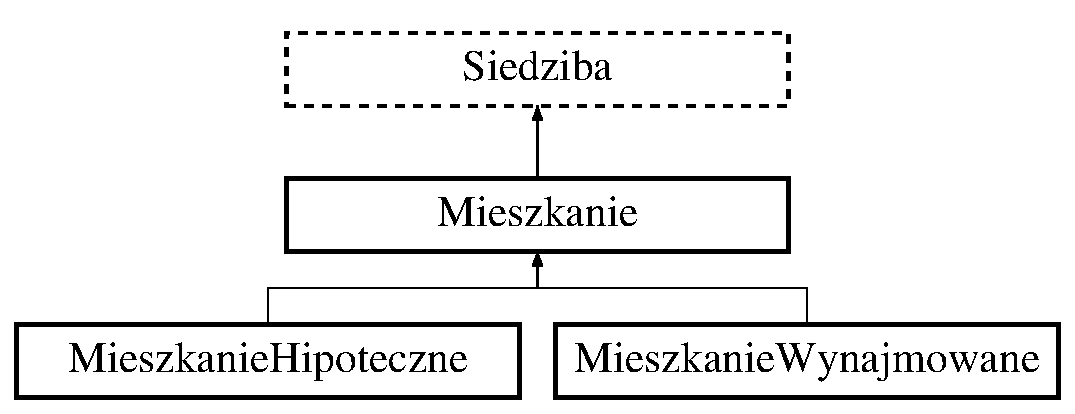
\includegraphics[height=3.000000cm]{class_mieszkanie}
\end{center}
\end{figure}
\subsection*{Public Member Functions}
\begin{DoxyCompactItemize}
\item 
\hyperlink{class_mieszkanie_a2c48251c70dd72049d77bdfa9f506355}{Mieszkanie} ()\hypertarget{class_mieszkanie_a2c48251c70dd72049d77bdfa9f506355}{}\label{class_mieszkanie_a2c48251c70dd72049d77bdfa9f506355}

\begin{DoxyCompactList}\small\item\em Konstruktor. \end{DoxyCompactList}\item 
\hyperlink{class_mieszkanie_ad42e3ad03375cec028c743febdb939d9}{Mieszkanie} (const \hyperlink{class_mieszkanie}{Mieszkanie} \&orig)\hypertarget{class_mieszkanie_ad42e3ad03375cec028c743febdb939d9}{}\label{class_mieszkanie_ad42e3ad03375cec028c743febdb939d9}

\begin{DoxyCompactList}\small\item\em Konstruktor kopiujacy. \end{DoxyCompactList}\item 
\hyperlink{class_mieszkanie_af324f74a786489b6850d7130200420de}{$\sim$\+Mieszkanie} ()\hypertarget{class_mieszkanie_af324f74a786489b6850d7130200420de}{}\label{class_mieszkanie_af324f74a786489b6850d7130200420de}

\begin{DoxyCompactList}\small\item\em Destruktor czyszczacy pamiec. \end{DoxyCompactList}\item 
bool \hyperlink{class_mieszkanie_ac328e12cf91e82575b9df90761eda765}{operator!=} (const \hyperlink{class_mieszkanie}{Mieszkanie} \&m2)
\begin{DoxyCompactList}\small\item\em Porownuje czy nie bylo juz danego wystapienia. \end{DoxyCompactList}\item 
virtual void \hyperlink{class_mieszkanie_ae4d42bcda6f9d88dd22fdc5e8d6f3072}{wirtualna} ()
\item 
void \hyperlink{class_mieszkanie_a0e2991b16dbe087b360747e20772e2a3}{Przeciaz\+Mnie} ()
\end{DoxyCompactItemize}
\subsection*{Public Attributes}
\begin{DoxyCompactItemize}
\item 
string {\bfseries nazw\+Wlasciciela}\hypertarget{class_mieszkanie_ab23f8abec3a1366d04f8d5094d732c2f}{}\label{class_mieszkanie_ab23f8abec3a1366d04f8d5094d732c2f}

\item 
float {\bfseries powierzchnia}\hypertarget{class_mieszkanie_a422cafa9d46454798553657ef1701b55}{}\label{class_mieszkanie_a422cafa9d46454798553657ef1701b55}

\item 
int {\bfseries liczba\+Pokoi}\hypertarget{class_mieszkanie_aaf00f775428df4b565804d71f9c65da0}{}\label{class_mieszkanie_aaf00f775428df4b565804d71f9c65da0}

\item 
bool {\bfseries zamieszkane}\hypertarget{class_mieszkanie_aff64593cdcbf15d53f535d1a32f09332}{}\label{class_mieszkanie_aff64593cdcbf15d53f535d1a32f09332}

\end{DoxyCompactItemize}
\subsection*{Static Public Attributes}
\begin{DoxyCompactItemize}
\item 
static unsigned {\bfseries liczba\+Wczytanych\+Mieszk} = 0\hypertarget{class_mieszkanie_a3a33bdd1910bff7f953e56d6ec16de07}{}\label{class_mieszkanie_a3a33bdd1910bff7f953e56d6ec16de07}

\end{DoxyCompactItemize}
\subsection*{Additional Inherited Members}


\subsection{Detailed Description}
Klasa reprezentujaca mieszkanie. 

\subsection{Member Function Documentation}
\index{Mieszkanie@{Mieszkanie}!operator"!=@{operator"!=}}
\index{operator"!=@{operator"!=}!Mieszkanie@{Mieszkanie}}
\subsubsection[{\texorpdfstring{operator"!=(const Mieszkanie \&m2)}{operator!=(const Mieszkanie &m2)}}]{\setlength{\rightskip}{0pt plus 5cm}bool Mieszkanie\+::operator!= (
\begin{DoxyParamCaption}
\item[{const {\bf Mieszkanie} \&}]{m2}
\end{DoxyParamCaption}
)\hspace{0.3cm}{\ttfamily [inline]}}\hypertarget{class_mieszkanie_ac328e12cf91e82575b9df90761eda765}{}\label{class_mieszkanie_ac328e12cf91e82575b9df90761eda765}


Porownuje czy nie bylo juz danego wystapienia. 


\begin{DoxyParams}{Parameters}
{\em Obiekt} & \\
\hline
\end{DoxyParams}
\begin{DoxyReturn}{Returns}
Prawde jesli warunki zostaly spelnione w przeciwnym przypadku falsz 
\end{DoxyReturn}
\index{Mieszkanie@{Mieszkanie}!Przeciaz\+Mnie@{Przeciaz\+Mnie}}
\index{Przeciaz\+Mnie@{Przeciaz\+Mnie}!Mieszkanie@{Mieszkanie}}
\subsubsection[{\texorpdfstring{Przeciaz\+Mnie()}{PrzeciazMnie()}}]{\setlength{\rightskip}{0pt plus 5cm}void Mieszkanie\+::\+Przeciaz\+Mnie (
\begin{DoxyParamCaption}
{}
\end{DoxyParamCaption}
)\hspace{0.3cm}{\ttfamily [virtual]}}\hypertarget{class_mieszkanie_a0e2991b16dbe087b360747e20772e2a3}{}\label{class_mieszkanie_a0e2991b16dbe087b360747e20772e2a3}
metoda czysto wirtualna przeciazana w mieszkaniu -\/ dla pokazania 

Implements \hyperlink{class_siedziba_aaaf836dbc2a5cb5afa25da87bc178a1c}{Siedziba}.



Reimplemented in \hyperlink{class_mieszkanie_wynajmowane_a1e7ec6bae620de2793c395b9a99feec8}{Mieszkanie\+Wynajmowane}, and \hyperlink{class_mieszkanie_hipoteczne_a54b4efeba76c6f179e4f1d5331892c2c}{Mieszkanie\+Hipoteczne}.

\index{Mieszkanie@{Mieszkanie}!wirtualna@{wirtualna}}
\index{wirtualna@{wirtualna}!Mieszkanie@{Mieszkanie}}
\subsubsection[{\texorpdfstring{wirtualna()}{wirtualna()}}]{\setlength{\rightskip}{0pt plus 5cm}void Mieszkanie\+::wirtualna (
\begin{DoxyParamCaption}
{}
\end{DoxyParamCaption}
)\hspace{0.3cm}{\ttfamily [virtual]}}\hypertarget{class_mieszkanie_ae4d42bcda6f9d88dd22fdc5e8d6f3072}{}\label{class_mieszkanie_ae4d42bcda6f9d88dd22fdc5e8d6f3072}
metoda wirtualna w mieszkaniu -\/ dla pokazania 

Reimplemented from \hyperlink{class_siedziba_a263f6218be66b3291c2cc7c8b1c0ec07}{Siedziba}.



The documentation for this class was generated from the following files\+:\begin{DoxyCompactItemize}
\item 
Mieszkanie.\+h\item 
Mieszkanie.\+cpp\end{DoxyCompactItemize}

\hypertarget{class_mieszkanie_hipoteczne}{}\section{Mieszkanie\+Hipoteczne Class Reference}
\label{class_mieszkanie_hipoteczne}\index{Mieszkanie\+Hipoteczne@{Mieszkanie\+Hipoteczne}}


Klasa \hyperlink{class_mieszkanie_hipoteczne}{Mieszkanie\+Hipoteczne}.  




{\ttfamily \#include $<$Mieszkanie\+Hipoteczne.\+h$>$}

Inheritance diagram for Mieszkanie\+Hipoteczne\+:\begin{figure}[H]
\begin{center}
\leavevmode
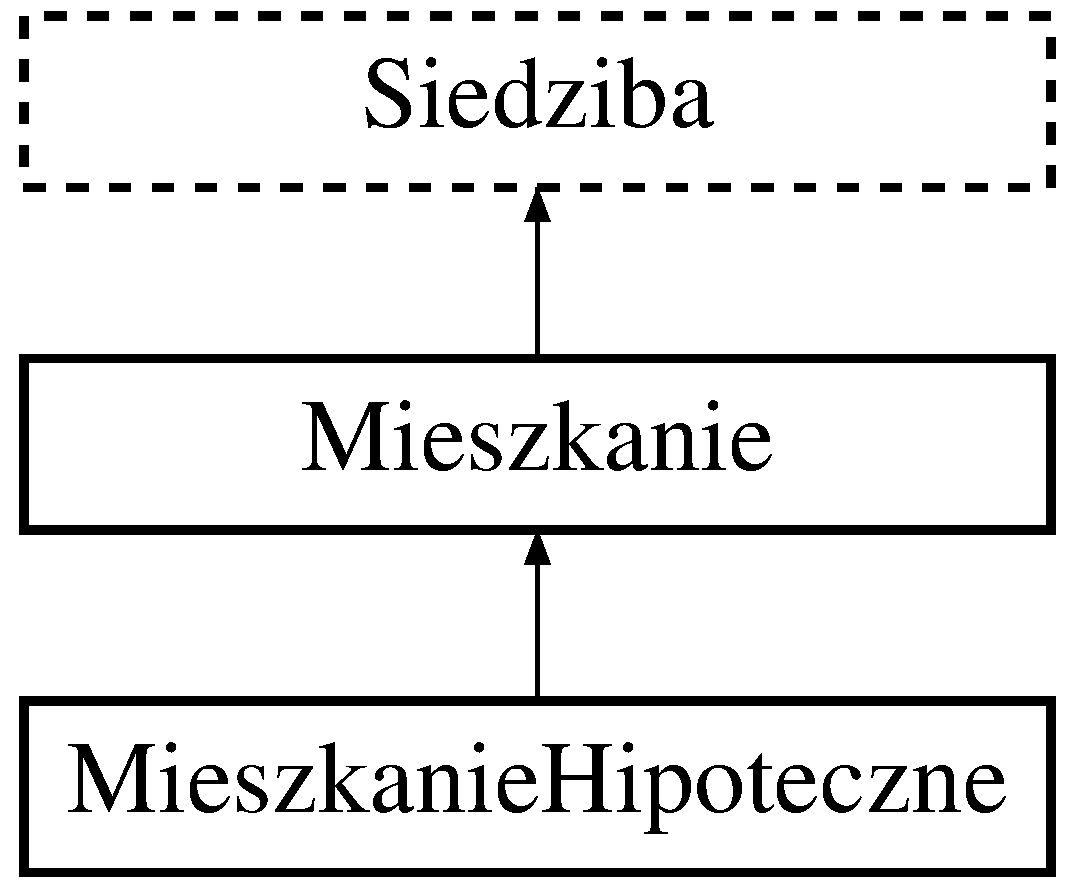
\includegraphics[height=3.000000cm]{class_mieszkanie_hipoteczne}
\end{center}
\end{figure}
\subsection*{Public Member Functions}
\begin{DoxyCompactItemize}
\item 
\hyperlink{class_mieszkanie_hipoteczne_aaa29d6a57a58d5993272f2a33c1bcad4}{Mieszkanie\+Hipoteczne} ()
\item 
virtual \hyperlink{class_mieszkanie_hipoteczne_a5e60ac18ab28467e23c0c4c980d48808}{$\sim$\+Mieszkanie\+Hipoteczne} ()
\item 
\hyperlink{class_mieszkanie_hipoteczne_ac79bd832402d66069d71ca1ca194af21}{Mieszkanie\+Hipoteczne} (const \hyperlink{class_mieszkanie_hipoteczne}{Mieszkanie\+Hipoteczne} \&other)
\item 
\hyperlink{class_mieszkanie_hipoteczne}{Mieszkanie\+Hipoteczne} \& \hyperlink{class_mieszkanie_hipoteczne_ae07e5624429cac150e407919d23f71cd}{operator=} (const \hyperlink{class_mieszkanie_hipoteczne}{Mieszkanie\+Hipoteczne} \&other)
\item 
float \hyperlink{class_mieszkanie_hipoteczne_ac4b1e687881c20d9caa088fc8fe65257}{Get\+Podatek} ()
\item 
void \hyperlink{class_mieszkanie_hipoteczne_a57729af61fa1b75f452d6f4a1199338b}{Set\+Podatek} (float val)
\item 
void \hyperlink{class_mieszkanie_hipoteczne_a54b4efeba76c6f179e4f1d5331892c2c}{Przeciaz\+Mnie} ()
\end{DoxyCompactItemize}
\subsection*{Additional Inherited Members}


\subsection{Detailed Description}
Klasa \hyperlink{class_mieszkanie_hipoteczne}{Mieszkanie\+Hipoteczne}. 

\subsection{Constructor \& Destructor Documentation}
\index{Mieszkanie\+Hipoteczne@{Mieszkanie\+Hipoteczne}!Mieszkanie\+Hipoteczne@{Mieszkanie\+Hipoteczne}}
\index{Mieszkanie\+Hipoteczne@{Mieszkanie\+Hipoteczne}!Mieszkanie\+Hipoteczne@{Mieszkanie\+Hipoteczne}}
\subsubsection[{\texorpdfstring{Mieszkanie\+Hipoteczne()}{MieszkanieHipoteczne()}}]{\setlength{\rightskip}{0pt plus 5cm}Mieszkanie\+Hipoteczne\+::\+Mieszkanie\+Hipoteczne (
\begin{DoxyParamCaption}
{}
\end{DoxyParamCaption}
)}\hypertarget{class_mieszkanie_hipoteczne_aaa29d6a57a58d5993272f2a33c1bcad4}{}\label{class_mieszkanie_hipoteczne_aaa29d6a57a58d5993272f2a33c1bcad4}
Konstruktor \index{Mieszkanie\+Hipoteczne@{Mieszkanie\+Hipoteczne}!````~Mieszkanie\+Hipoteczne@{$\sim$\+Mieszkanie\+Hipoteczne}}
\index{````~Mieszkanie\+Hipoteczne@{$\sim$\+Mieszkanie\+Hipoteczne}!Mieszkanie\+Hipoteczne@{Mieszkanie\+Hipoteczne}}
\subsubsection[{\texorpdfstring{$\sim$\+Mieszkanie\+Hipoteczne()}{~MieszkanieHipoteczne()}}]{\setlength{\rightskip}{0pt plus 5cm}Mieszkanie\+Hipoteczne\+::$\sim$\+Mieszkanie\+Hipoteczne (
\begin{DoxyParamCaption}
{}
\end{DoxyParamCaption}
)\hspace{0.3cm}{\ttfamily [virtual]}}\hypertarget{class_mieszkanie_hipoteczne_a5e60ac18ab28467e23c0c4c980d48808}{}\label{class_mieszkanie_hipoteczne_a5e60ac18ab28467e23c0c4c980d48808}
Destruktor \index{Mieszkanie\+Hipoteczne@{Mieszkanie\+Hipoteczne}!Mieszkanie\+Hipoteczne@{Mieszkanie\+Hipoteczne}}
\index{Mieszkanie\+Hipoteczne@{Mieszkanie\+Hipoteczne}!Mieszkanie\+Hipoteczne@{Mieszkanie\+Hipoteczne}}
\subsubsection[{\texorpdfstring{Mieszkanie\+Hipoteczne(const Mieszkanie\+Hipoteczne \&other)}{MieszkanieHipoteczne(const MieszkanieHipoteczne &other)}}]{\setlength{\rightskip}{0pt plus 5cm}Mieszkanie\+Hipoteczne\+::\+Mieszkanie\+Hipoteczne (
\begin{DoxyParamCaption}
\item[{const {\bf Mieszkanie\+Hipoteczne} \&}]{other}
\end{DoxyParamCaption}
)}\hypertarget{class_mieszkanie_hipoteczne_ac79bd832402d66069d71ca1ca194af21}{}\label{class_mieszkanie_hipoteczne_ac79bd832402d66069d71ca1ca194af21}
Konstruktor kopiujacy 
\begin{DoxyParams}{Parameters}
{\em obiekt} & do skopiowania \\
\hline
\end{DoxyParams}


\subsection{Member Function Documentation}
\index{Mieszkanie\+Hipoteczne@{Mieszkanie\+Hipoteczne}!Get\+Podatek@{Get\+Podatek}}
\index{Get\+Podatek@{Get\+Podatek}!Mieszkanie\+Hipoteczne@{Mieszkanie\+Hipoteczne}}
\subsubsection[{\texorpdfstring{Get\+Podatek()}{GetPodatek()}}]{\setlength{\rightskip}{0pt plus 5cm}float Mieszkanie\+Hipoteczne\+::\+Get\+Podatek (
\begin{DoxyParamCaption}
{}
\end{DoxyParamCaption}
)\hspace{0.3cm}{\ttfamily [inline]}}\hypertarget{class_mieszkanie_hipoteczne_ac4b1e687881c20d9caa088fc8fe65257}{}\label{class_mieszkanie_hipoteczne_ac4b1e687881c20d9caa088fc8fe65257}
Dostep do podatku \begin{DoxyReturn}{Returns}
Obecna wartosc podatku 
\end{DoxyReturn}
\index{Mieszkanie\+Hipoteczne@{Mieszkanie\+Hipoteczne}!operator=@{operator=}}
\index{operator=@{operator=}!Mieszkanie\+Hipoteczne@{Mieszkanie\+Hipoteczne}}
\subsubsection[{\texorpdfstring{operator=(const Mieszkanie\+Hipoteczne \&other)}{operator=(const MieszkanieHipoteczne &other)}}]{\setlength{\rightskip}{0pt plus 5cm}{\bf Mieszkanie\+Hipoteczne} \& Mieszkanie\+Hipoteczne\+::operator= (
\begin{DoxyParamCaption}
\item[{const {\bf Mieszkanie\+Hipoteczne} \&}]{other}
\end{DoxyParamCaption}
)}\hypertarget{class_mieszkanie_hipoteczne_ae07e5624429cac150e407919d23f71cd}{}\label{class_mieszkanie_hipoteczne_ae07e5624429cac150e407919d23f71cd}
Operator przypisania 
\begin{DoxyParams}{Parameters}
{\em inny} & obiekt do przypisania od \\
\hline
\end{DoxyParams}
\begin{DoxyReturn}{Returns}
Referencja do niego 
\end{DoxyReturn}
\index{Mieszkanie\+Hipoteczne@{Mieszkanie\+Hipoteczne}!Przeciaz\+Mnie@{Przeciaz\+Mnie}}
\index{Przeciaz\+Mnie@{Przeciaz\+Mnie}!Mieszkanie\+Hipoteczne@{Mieszkanie\+Hipoteczne}}
\subsubsection[{\texorpdfstring{Przeciaz\+Mnie()}{PrzeciazMnie()}}]{\setlength{\rightskip}{0pt plus 5cm}void Mieszkanie\+Hipoteczne\+::\+Przeciaz\+Mnie (
\begin{DoxyParamCaption}
{}
\end{DoxyParamCaption}
)\hspace{0.3cm}{\ttfamily [inline]}, {\ttfamily [virtual]}}\hypertarget{class_mieszkanie_hipoteczne_a54b4efeba76c6f179e4f1d5331892c2c}{}\label{class_mieszkanie_hipoteczne_a54b4efeba76c6f179e4f1d5331892c2c}
metoda czysto wirtualna przeciazana w mieszkaniuhipotecznym -\/ dla pokazania 

Reimplemented from \hyperlink{class_mieszkanie_a0e2991b16dbe087b360747e20772e2a3}{Mieszkanie}.

\index{Mieszkanie\+Hipoteczne@{Mieszkanie\+Hipoteczne}!Set\+Podatek@{Set\+Podatek}}
\index{Set\+Podatek@{Set\+Podatek}!Mieszkanie\+Hipoteczne@{Mieszkanie\+Hipoteczne}}
\subsubsection[{\texorpdfstring{Set\+Podatek(float val)}{SetPodatek(float val)}}]{\setlength{\rightskip}{0pt plus 5cm}void Mieszkanie\+Hipoteczne\+::\+Set\+Podatek (
\begin{DoxyParamCaption}
\item[{float}]{val}
\end{DoxyParamCaption}
)\hspace{0.3cm}{\ttfamily [inline]}}\hypertarget{class_mieszkanie_hipoteczne_a57729af61fa1b75f452d6f4a1199338b}{}\label{class_mieszkanie_hipoteczne_a57729af61fa1b75f452d6f4a1199338b}
Ustaw wartosc podatku 
\begin{DoxyParams}{Parameters}
{\em val} & \\
\hline
\end{DoxyParams}


The documentation for this class was generated from the following files\+:\begin{DoxyCompactItemize}
\item 
Mieszkanie\+Hipoteczne.\+h\item 
Mieszkanie\+Hipoteczne.\+cpp\end{DoxyCompactItemize}

\hypertarget{class_mieszkanie_wynajmowane}{}\section{Mieszkanie\+Wynajmowane Class Reference}
\label{class_mieszkanie_wynajmowane}\index{Mieszkanie\+Wynajmowane@{Mieszkanie\+Wynajmowane}}


Klasa \hyperlink{class_mieszkanie_wynajmowane}{Mieszkanie\+Wynajmowane}.  




{\ttfamily \#include $<$Mieszkanie\+Wynajmowane.\+h$>$}

Inheritance diagram for Mieszkanie\+Wynajmowane\+:\begin{figure}[H]
\begin{center}
\leavevmode
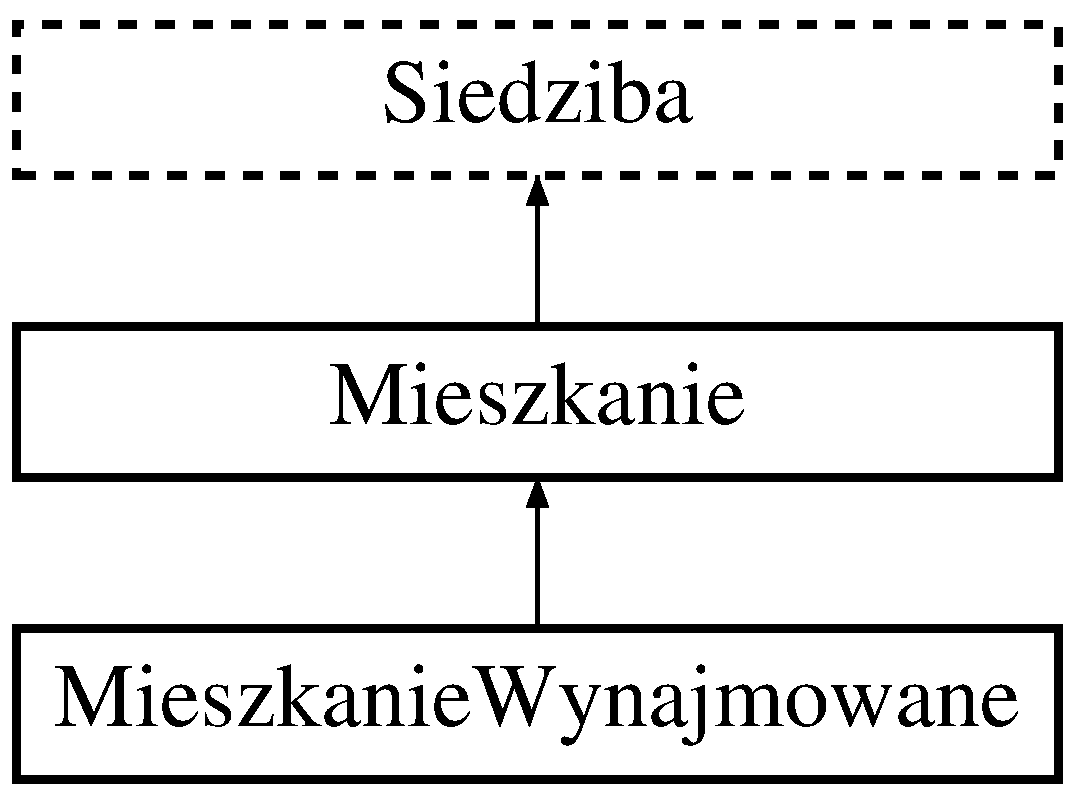
\includegraphics[height=3.000000cm]{class_mieszkanie_wynajmowane}
\end{center}
\end{figure}
\subsection*{Public Member Functions}
\begin{DoxyCompactItemize}
\item 
\hyperlink{class_mieszkanie_wynajmowane_a8f23bf351540b25870d8816097e49c79}{Mieszkanie\+Wynajmowane} ()
\item 
virtual \hyperlink{class_mieszkanie_wynajmowane_ac08918efc1caebf86cb3eb54a8b14654}{$\sim$\+Mieszkanie\+Wynajmowane} ()
\item 
\hyperlink{class_mieszkanie_wynajmowane_a5f45599654f50e91e39f655aea84ccc3}{Mieszkanie\+Wynajmowane} (const \hyperlink{class_mieszkanie_wynajmowane}{Mieszkanie\+Wynajmowane} \&other)
\item 
\hyperlink{class_mieszkanie_wynajmowane}{Mieszkanie\+Wynajmowane} \& \hyperlink{class_mieszkanie_wynajmowane_a41c2c74090f7902b1277b5ec1b6fea4b}{operator=} (const \hyperlink{class_mieszkanie_wynajmowane}{Mieszkanie\+Wynajmowane} \&other)
\item 
float \hyperlink{class_mieszkanie_wynajmowane_af74eb718c87bc697522c3006d153464f}{Get\+Czynsz} ()
\item 
void \hyperlink{class_mieszkanie_wynajmowane_a54744a366a938cab96ae6e542e1770be}{Set\+Czynsz} (float val)
\item 
string \hyperlink{class_mieszkanie_wynajmowane_a8bdb7570f577836e8cf443ecccb23476}{Getnazw\+Wynajmujacego} ()
\item 
void \hyperlink{class_mieszkanie_wynajmowane_a964628ec1b2f577e7ea7c8de51b9426f}{Setnazw\+Wynajmujacego} (string val)
\item 
void \hyperlink{class_mieszkanie_wynajmowane_a1e7ec6bae620de2793c395b9a99feec8}{Przeciaz\+Mnie} ()
\end{DoxyCompactItemize}
\subsection*{Friends}
\begin{DoxyCompactItemize}
\item 
ostream \& {\bfseries operator$<$$<$} (ostream \&s, const \hyperlink{class_mieszkanie_wynajmowane}{Mieszkanie\+Wynajmowane} \&m)\hypertarget{class_mieszkanie_wynajmowane_a1e0b9dd9eae2f5c6f4bb6464c7193c84}{}\label{class_mieszkanie_wynajmowane_a1e0b9dd9eae2f5c6f4bb6464c7193c84}

\item 
istream \& {\bfseries operator$>$$>$} (istream \&s, \hyperlink{class_mieszkanie_wynajmowane}{Mieszkanie\+Wynajmowane} \&m)\hypertarget{class_mieszkanie_wynajmowane_aa99319125a0e2f04a1c230c0572626ae}{}\label{class_mieszkanie_wynajmowane_aa99319125a0e2f04a1c230c0572626ae}

\end{DoxyCompactItemize}
\subsection*{Additional Inherited Members}


\subsection{Detailed Description}
Klasa \hyperlink{class_mieszkanie_wynajmowane}{Mieszkanie\+Wynajmowane}. 

\subsection{Constructor \& Destructor Documentation}
\index{Mieszkanie\+Wynajmowane@{Mieszkanie\+Wynajmowane}!Mieszkanie\+Wynajmowane@{Mieszkanie\+Wynajmowane}}
\index{Mieszkanie\+Wynajmowane@{Mieszkanie\+Wynajmowane}!Mieszkanie\+Wynajmowane@{Mieszkanie\+Wynajmowane}}
\subsubsection[{\texorpdfstring{Mieszkanie\+Wynajmowane()}{MieszkanieWynajmowane()}}]{\setlength{\rightskip}{0pt plus 5cm}Mieszkanie\+Wynajmowane\+::\+Mieszkanie\+Wynajmowane (
\begin{DoxyParamCaption}
{}
\end{DoxyParamCaption}
)}\hypertarget{class_mieszkanie_wynajmowane_a8f23bf351540b25870d8816097e49c79}{}\label{class_mieszkanie_wynajmowane_a8f23bf351540b25870d8816097e49c79}
Konstructor \index{Mieszkanie\+Wynajmowane@{Mieszkanie\+Wynajmowane}!````~Mieszkanie\+Wynajmowane@{$\sim$\+Mieszkanie\+Wynajmowane}}
\index{````~Mieszkanie\+Wynajmowane@{$\sim$\+Mieszkanie\+Wynajmowane}!Mieszkanie\+Wynajmowane@{Mieszkanie\+Wynajmowane}}
\subsubsection[{\texorpdfstring{$\sim$\+Mieszkanie\+Wynajmowane()}{~MieszkanieWynajmowane()}}]{\setlength{\rightskip}{0pt plus 5cm}Mieszkanie\+Wynajmowane\+::$\sim$\+Mieszkanie\+Wynajmowane (
\begin{DoxyParamCaption}
{}
\end{DoxyParamCaption}
)\hspace{0.3cm}{\ttfamily [virtual]}}\hypertarget{class_mieszkanie_wynajmowane_ac08918efc1caebf86cb3eb54a8b14654}{}\label{class_mieszkanie_wynajmowane_ac08918efc1caebf86cb3eb54a8b14654}
Destructor \index{Mieszkanie\+Wynajmowane@{Mieszkanie\+Wynajmowane}!Mieszkanie\+Wynajmowane@{Mieszkanie\+Wynajmowane}}
\index{Mieszkanie\+Wynajmowane@{Mieszkanie\+Wynajmowane}!Mieszkanie\+Wynajmowane@{Mieszkanie\+Wynajmowane}}
\subsubsection[{\texorpdfstring{Mieszkanie\+Wynajmowane(const Mieszkanie\+Wynajmowane \&other)}{MieszkanieWynajmowane(const MieszkanieWynajmowane &other)}}]{\setlength{\rightskip}{0pt plus 5cm}Mieszkanie\+Wynajmowane\+::\+Mieszkanie\+Wynajmowane (
\begin{DoxyParamCaption}
\item[{const {\bf Mieszkanie\+Wynajmowane} \&}]{other}
\end{DoxyParamCaption}
)}\hypertarget{class_mieszkanie_wynajmowane_a5f45599654f50e91e39f655aea84ccc3}{}\label{class_mieszkanie_wynajmowane_a5f45599654f50e91e39f655aea84ccc3}
Konstruktor kopiujacy 
\begin{DoxyParams}{Parameters}
{\em inny} & obiekt do kopiowania \\
\hline
\end{DoxyParams}


\subsection{Member Function Documentation}
\index{Mieszkanie\+Wynajmowane@{Mieszkanie\+Wynajmowane}!Get\+Czynsz@{Get\+Czynsz}}
\index{Get\+Czynsz@{Get\+Czynsz}!Mieszkanie\+Wynajmowane@{Mieszkanie\+Wynajmowane}}
\subsubsection[{\texorpdfstring{Get\+Czynsz()}{GetCzynsz()}}]{\setlength{\rightskip}{0pt plus 5cm}float Mieszkanie\+Wynajmowane\+::\+Get\+Czynsz (
\begin{DoxyParamCaption}
{}
\end{DoxyParamCaption}
)\hspace{0.3cm}{\ttfamily [inline]}}\hypertarget{class_mieszkanie_wynajmowane_af74eb718c87bc697522c3006d153464f}{}\label{class_mieszkanie_wynajmowane_af74eb718c87bc697522c3006d153464f}
Dostep do czynszu \begin{DoxyReturn}{Returns}
Obecna wartosc czynszu 
\end{DoxyReturn}
\index{Mieszkanie\+Wynajmowane@{Mieszkanie\+Wynajmowane}!Getnazw\+Wynajmujacego@{Getnazw\+Wynajmujacego}}
\index{Getnazw\+Wynajmujacego@{Getnazw\+Wynajmujacego}!Mieszkanie\+Wynajmowane@{Mieszkanie\+Wynajmowane}}
\subsubsection[{\texorpdfstring{Getnazw\+Wynajmujacego()}{GetnazwWynajmujacego()}}]{\setlength{\rightskip}{0pt plus 5cm}string Mieszkanie\+Wynajmowane\+::\+Getnazw\+Wynajmujacego (
\begin{DoxyParamCaption}
{}
\end{DoxyParamCaption}
)\hspace{0.3cm}{\ttfamily [inline]}}\hypertarget{class_mieszkanie_wynajmowane_a8bdb7570f577836e8cf443ecccb23476}{}\label{class_mieszkanie_wynajmowane_a8bdb7570f577836e8cf443ecccb23476}
Dostep do nazwy wynajmujacego \begin{DoxyReturn}{Returns}
Obecna nazwa wynajmujacego 
\end{DoxyReturn}
\index{Mieszkanie\+Wynajmowane@{Mieszkanie\+Wynajmowane}!operator=@{operator=}}
\index{operator=@{operator=}!Mieszkanie\+Wynajmowane@{Mieszkanie\+Wynajmowane}}
\subsubsection[{\texorpdfstring{operator=(const Mieszkanie\+Wynajmowane \&other)}{operator=(const MieszkanieWynajmowane &other)}}]{\setlength{\rightskip}{0pt plus 5cm}{\bf Mieszkanie\+Wynajmowane} \& Mieszkanie\+Wynajmowane\+::operator= (
\begin{DoxyParamCaption}
\item[{const {\bf Mieszkanie\+Wynajmowane} \&}]{other}
\end{DoxyParamCaption}
)}\hypertarget{class_mieszkanie_wynajmowane_a41c2c74090f7902b1277b5ec1b6fea4b}{}\label{class_mieszkanie_wynajmowane_a41c2c74090f7902b1277b5ec1b6fea4b}
Operator przypisania 
\begin{DoxyParams}{Parameters}
{\em inny} & obiekt do przypisania od \\
\hline
\end{DoxyParams}
\begin{DoxyReturn}{Returns}
Referencja do niego 
\end{DoxyReturn}
\index{Mieszkanie\+Wynajmowane@{Mieszkanie\+Wynajmowane}!Przeciaz\+Mnie@{Przeciaz\+Mnie}}
\index{Przeciaz\+Mnie@{Przeciaz\+Mnie}!Mieszkanie\+Wynajmowane@{Mieszkanie\+Wynajmowane}}
\subsubsection[{\texorpdfstring{Przeciaz\+Mnie()}{PrzeciazMnie()}}]{\setlength{\rightskip}{0pt plus 5cm}void Mieszkanie\+Wynajmowane\+::\+Przeciaz\+Mnie (
\begin{DoxyParamCaption}
{}
\end{DoxyParamCaption}
)\hspace{0.3cm}{\ttfamily [inline]}, {\ttfamily [virtual]}}\hypertarget{class_mieszkanie_wynajmowane_a1e7ec6bae620de2793c395b9a99feec8}{}\label{class_mieszkanie_wynajmowane_a1e7ec6bae620de2793c395b9a99feec8}
metoda czysto wirtualna przeciazana w mieszkaniu wynajmowanym -\/ dla pokazania 

Reimplemented from \hyperlink{class_mieszkanie_a0e2991b16dbe087b360747e20772e2a3}{Mieszkanie}.

\index{Mieszkanie\+Wynajmowane@{Mieszkanie\+Wynajmowane}!Set\+Czynsz@{Set\+Czynsz}}
\index{Set\+Czynsz@{Set\+Czynsz}!Mieszkanie\+Wynajmowane@{Mieszkanie\+Wynajmowane}}
\subsubsection[{\texorpdfstring{Set\+Czynsz(float val)}{SetCzynsz(float val)}}]{\setlength{\rightskip}{0pt plus 5cm}void Mieszkanie\+Wynajmowane\+::\+Set\+Czynsz (
\begin{DoxyParamCaption}
\item[{float}]{val}
\end{DoxyParamCaption}
)\hspace{0.3cm}{\ttfamily [inline]}}\hypertarget{class_mieszkanie_wynajmowane_a54744a366a938cab96ae6e542e1770be}{}\label{class_mieszkanie_wynajmowane_a54744a366a938cab96ae6e542e1770be}
Ustaw czynsz 
\begin{DoxyParams}{Parameters}
{\em val} & \\
\hline
\end{DoxyParams}
\index{Mieszkanie\+Wynajmowane@{Mieszkanie\+Wynajmowane}!Setnazw\+Wynajmujacego@{Setnazw\+Wynajmujacego}}
\index{Setnazw\+Wynajmujacego@{Setnazw\+Wynajmujacego}!Mieszkanie\+Wynajmowane@{Mieszkanie\+Wynajmowane}}
\subsubsection[{\texorpdfstring{Setnazw\+Wynajmujacego(string val)}{SetnazwWynajmujacego(string val)}}]{\setlength{\rightskip}{0pt plus 5cm}void Mieszkanie\+Wynajmowane\+::\+Setnazw\+Wynajmujacego (
\begin{DoxyParamCaption}
\item[{string}]{val}
\end{DoxyParamCaption}
)\hspace{0.3cm}{\ttfamily [inline]}}\hypertarget{class_mieszkanie_wynajmowane_a964628ec1b2f577e7ea7c8de51b9426f}{}\label{class_mieszkanie_wynajmowane_a964628ec1b2f577e7ea7c8de51b9426f}
Ustaw nazwe wynajmujacego 
\begin{DoxyParams}{Parameters}
{\em val} & \\
\hline
\end{DoxyParams}


The documentation for this class was generated from the following files\+:\begin{DoxyCompactItemize}
\item 
Mieszkanie\+Wynajmowane.\+h\item 
Mieszkanie\+Wynajmowane.\+cpp\end{DoxyCompactItemize}

\hypertarget{class_siedziba}{}\section{Siedziba Class Reference}
\label{class_siedziba}\index{Siedziba@{Siedziba}}


Klasa abstrakcyjna \hyperlink{class_siedziba}{Siedziba}.  




{\ttfamily \#include $<$Siedziba.\+h$>$}

Inheritance diagram for Siedziba\+:\begin{figure}[H]
\begin{center}
\leavevmode
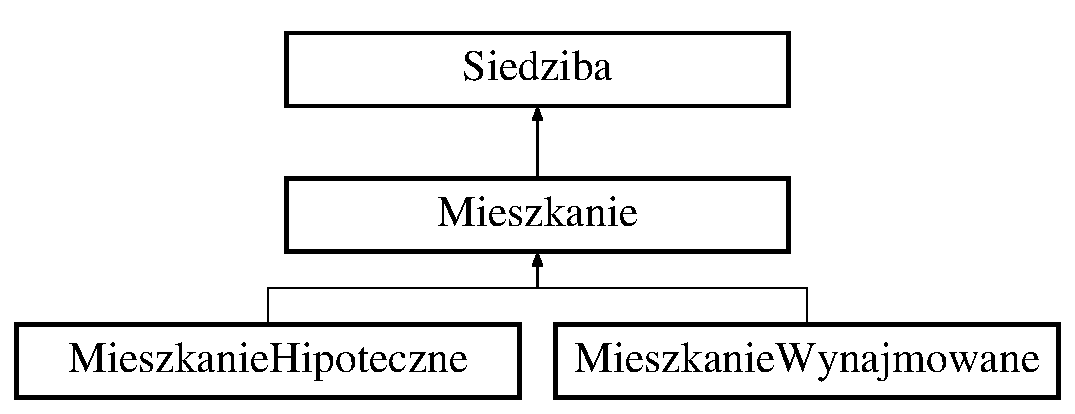
\includegraphics[height=3.000000cm]{class_siedziba}
\end{center}
\end{figure}
\subsection*{Public Member Functions}
\begin{DoxyCompactItemize}
\item 
\hyperlink{class_siedziba_a3d2babb95b8eae60c04eb73c9db0981c}{Siedziba} ()
\item 
virtual \hyperlink{class_siedziba_a1dc3fee9549a390981000aa8df28ee1e}{$\sim$\+Siedziba} ()
\item 
string \hyperlink{class_siedziba_a91a27ef9059b4984bdbc32baa5803bf3}{Get\+Adres} ()
\item 
void \hyperlink{class_siedziba_a93fede127dbc0264f7c31f3ea5059107}{Set\+Adres} (string val)
\item 
virtual void \hyperlink{class_siedziba_a263f6218be66b3291c2cc7c8b1c0ec07}{wirtualna} ()
\item 
virtual void \hyperlink{class_siedziba_aaaf836dbc2a5cb5afa25da87bc178a1c}{Przeciaz\+Mnie} ()=0
\end{DoxyCompactItemize}
\subsection*{Protected Attributes}
\begin{DoxyCompactItemize}
\item 
string \hyperlink{class_siedziba_a049d7c2791bac5877eb2133319197277}{Adres}\hypertarget{class_siedziba_a049d7c2791bac5877eb2133319197277}{}\label{class_siedziba_a049d7c2791bac5877eb2133319197277}

\begin{DoxyCompactList}\small\item\em Glowna zmienna \char`\"{}\+Adres\char`\"{}. \end{DoxyCompactList}\end{DoxyCompactItemize}
\subsection*{Friends}
\begin{DoxyCompactItemize}
\item 
ostream \& \hyperlink{class_siedziba_a3baacc30876ca0af57072a89756f9be9}{operator$<$$<$} (ostream \&s, const \hyperlink{class_siedziba}{Siedziba} \&m)
\begin{DoxyCompactList}\small\item\em metoda czysto wirtualna \end{DoxyCompactList}\end{DoxyCompactItemize}


\subsection{Detailed Description}
Klasa abstrakcyjna \hyperlink{class_siedziba}{Siedziba}. 

\subsection{Constructor \& Destructor Documentation}
\index{Siedziba@{Siedziba}!Siedziba@{Siedziba}}
\index{Siedziba@{Siedziba}!Siedziba@{Siedziba}}
\subsubsection[{\texorpdfstring{Siedziba()}{Siedziba()}}]{\setlength{\rightskip}{0pt plus 5cm}Siedziba\+::\+Siedziba (
\begin{DoxyParamCaption}
{}
\end{DoxyParamCaption}
)}\hypertarget{class_siedziba_a3d2babb95b8eae60c04eb73c9db0981c}{}\label{class_siedziba_a3d2babb95b8eae60c04eb73c9db0981c}
Konstruktor \index{Siedziba@{Siedziba}!````~Siedziba@{$\sim$\+Siedziba}}
\index{````~Siedziba@{$\sim$\+Siedziba}!Siedziba@{Siedziba}}
\subsubsection[{\texorpdfstring{$\sim$\+Siedziba()}{~Siedziba()}}]{\setlength{\rightskip}{0pt plus 5cm}Siedziba\+::$\sim$\+Siedziba (
\begin{DoxyParamCaption}
{}
\end{DoxyParamCaption}
)\hspace{0.3cm}{\ttfamily [virtual]}}\hypertarget{class_siedziba_a1dc3fee9549a390981000aa8df28ee1e}{}\label{class_siedziba_a1dc3fee9549a390981000aa8df28ee1e}
Destruktor 

\subsection{Member Function Documentation}
\index{Siedziba@{Siedziba}!Get\+Adres@{Get\+Adres}}
\index{Get\+Adres@{Get\+Adres}!Siedziba@{Siedziba}}
\subsubsection[{\texorpdfstring{Get\+Adres()}{GetAdres()}}]{\setlength{\rightskip}{0pt plus 5cm}string Siedziba\+::\+Get\+Adres (
\begin{DoxyParamCaption}
{}
\end{DoxyParamCaption}
)\hspace{0.3cm}{\ttfamily [inline]}}\hypertarget{class_siedziba_a91a27ef9059b4984bdbc32baa5803bf3}{}\label{class_siedziba_a91a27ef9059b4984bdbc32baa5803bf3}
Dostep do Adresu \begin{DoxyReturn}{Returns}
Obecna wartosc adresu 
\end{DoxyReturn}
\index{Siedziba@{Siedziba}!Przeciaz\+Mnie@{Przeciaz\+Mnie}}
\index{Przeciaz\+Mnie@{Przeciaz\+Mnie}!Siedziba@{Siedziba}}
\subsubsection[{\texorpdfstring{Przeciaz\+Mnie()=0}{PrzeciazMnie()=0}}]{\setlength{\rightskip}{0pt plus 5cm}virtual void Siedziba\+::\+Przeciaz\+Mnie (
\begin{DoxyParamCaption}
{}
\end{DoxyParamCaption}
)\hspace{0.3cm}{\ttfamily [pure virtual]}}\hypertarget{class_siedziba_aaaf836dbc2a5cb5afa25da87bc178a1c}{}\label{class_siedziba_aaaf836dbc2a5cb5afa25da87bc178a1c}
metoda czysto wirtualna -\/ dla pokazania 

Implemented in \hyperlink{class_mieszkanie_wynajmowane_a1e7ec6bae620de2793c395b9a99feec8}{Mieszkanie\+Wynajmowane}, \hyperlink{class_mieszkanie_a0e2991b16dbe087b360747e20772e2a3}{Mieszkanie}, and \hyperlink{class_mieszkanie_hipoteczne_a54b4efeba76c6f179e4f1d5331892c2c}{Mieszkanie\+Hipoteczne}.

\index{Siedziba@{Siedziba}!Set\+Adres@{Set\+Adres}}
\index{Set\+Adres@{Set\+Adres}!Siedziba@{Siedziba}}
\subsubsection[{\texorpdfstring{Set\+Adres(string val)}{SetAdres(string val)}}]{\setlength{\rightskip}{0pt plus 5cm}void Siedziba\+::\+Set\+Adres (
\begin{DoxyParamCaption}
\item[{string}]{val}
\end{DoxyParamCaption}
)\hspace{0.3cm}{\ttfamily [inline]}}\hypertarget{class_siedziba_a93fede127dbc0264f7c31f3ea5059107}{}\label{class_siedziba_a93fede127dbc0264f7c31f3ea5059107}
Usaw Adres 
\begin{DoxyParams}{Parameters}
{\em val} & \\
\hline
\end{DoxyParams}
\index{Siedziba@{Siedziba}!wirtualna@{wirtualna}}
\index{wirtualna@{wirtualna}!Siedziba@{Siedziba}}
\subsubsection[{\texorpdfstring{wirtualna()}{wirtualna()}}]{\setlength{\rightskip}{0pt plus 5cm}virtual void Siedziba\+::wirtualna (
\begin{DoxyParamCaption}
{}
\end{DoxyParamCaption}
)\hspace{0.3cm}{\ttfamily [inline]}, {\ttfamily [virtual]}}\hypertarget{class_siedziba_a263f6218be66b3291c2cc7c8b1c0ec07}{}\label{class_siedziba_a263f6218be66b3291c2cc7c8b1c0ec07}
metoda wirtualna z siedziby -\/ dla pokazania 

Reimplemented in \hyperlink{class_mieszkanie_ae4d42bcda6f9d88dd22fdc5e8d6f3072}{Mieszkanie}.



\subsection{Friends And Related Function Documentation}
\index{Siedziba@{Siedziba}!operator$<$$<$@{operator$<$$<$}}
\index{operator$<$$<$@{operator$<$$<$}!Siedziba@{Siedziba}}
\subsubsection[{\texorpdfstring{operator$<$$<$}{operator<<}}]{\setlength{\rightskip}{0pt plus 5cm}ostream\& operator$<$$<$ (
\begin{DoxyParamCaption}
\item[{ostream \&}]{s, }
\item[{const {\bf Siedziba} \&}]{m}
\end{DoxyParamCaption}
)\hspace{0.3cm}{\ttfamily [friend]}}\hypertarget{class_siedziba_a3baacc30876ca0af57072a89756f9be9}{}\label{class_siedziba_a3baacc30876ca0af57072a89756f9be9}


metoda czysto wirtualna 

Przeciazenie operatora strumieniowego $<$$<$ 

The documentation for this class was generated from the following files\+:\begin{DoxyCompactItemize}
\item 
Siedziba.\+h\item 
Siedziba.\+cpp\end{DoxyCompactItemize}

%--- End generated contents ---

% Index
\backmatter
\newpage
\phantomsection
\clearemptydoublepage
\addcontentsline{toc}{chapter}{Index}
\printindex

\end{document}
